\documentclass[12pt,twoside]{article}

% La extensión total de la memoria deberá ser de un máximo de 50 páginas (excluidos resumen, índice y posibles anexos).

% Según las recomendaciones de estilo, el formato de la memoria se ajustará a lo siguiente:
% ? Formato del papel: DIN A4.
% ? Impresión a dos caras.
% ? Márgenes: superior e inferior, 2.5 cm. Márgenes laterales: páginas impares, izquierdo 4 cm y derecho 2 cm; páginas % pares, izquierdo 2 cm y derecho 4 cm.
% ? Tipo de letra: Times New Roman de 12 puntos.
% ? Interlineado: 1.5 líneas.
% ? Alineación: justificación completa.
% ? Sangrado de párrafo: 0.5 cm la primera línea de cada párrafo. No se
%pondrá espacio entre párrafos.
% ? Las páginas deberán ir numeradas en números arábigos.

% Teniendo en cuenta las indicaciones previas, definimos el estilo en LaTeX:

% Indicaciones para el idioma:
\usepackage[T1]{fontenc}
\usepackage[utf8]{inputenc}
\usepackage[spanish]{babel}

% Adaptación de itemize y enumerate a los usos tipograficos españoles:
\let\layoutspanish\relax
\addto\captionsspanish{\def\tablename{Tabla}} % para que escriba "Tabla" en lugar de "Cuadro"
\unaccentedoperators  % para que no acentúe los operadores

% Área de impresión de una página:
\usepackage[a4paper]{geometry}
  \geometry{hmargin={2.5cm,2.5cm},height=22cm}

% Formato de algunas distancias:
\renewcommand{\baselinestretch}{1.2}    % separación entre líneas de un mismo párrafo
\setlength{\partopsep}{0pt}
\setlength{\itemsep}{0pt}
\setlength{\topsep}{0pt}
\setlength{\parsep}{0pt}
\setlength{\parskip}{0.25\baselineskip}   % separación entre párrafos

\renewcommand{\textfraction}{0.1}   % mínima fracción de la página para el texto
\renewcommand{\topfraction}{1}      % máxima fracción de la página para objetos flotantes en la parte superior
\renewcommand{\bottomfraction}{1}
\renewcommand{\floatpagefraction}{1}

\setcounter{totalnumber}{5}
\setcounter{topnumber}{3}
\setcounter{bottomnumber}{2}

% Adaptación de las "caption" de los entorns "figure" y "table":
\usepackage{caption}
\setcaptionwidth{\textwidth}
\addtolength{\captionwidth}{-2\parindent}
\captionsetup{margin=\leftmargini,%
  width=\captionwidth,%
  labelfont={up,bf},%
  font={small,sl},%
  %indention={\captionindent
}

% Indentación del primer párrafo de una sección:
\usepackage{indentfirst}

% Definición del color grisclaro en la salida PDF:
\usepackage[pdftex]{color}

% Gráficos:
\usepackage[pdftex]{graphicx}

% Paquetes recomendados para la inclusión de fórmulas matemáticas:
\usepackage{amsmath}
\allowdisplaybreaks  % para que pueda partir fórmulas que ocupan más de una línea, necesita el paquete anterior
\usepackage{amssymb} % para cargar algunos símbolos como \blacksquare y \square
\usepackage{amsfonts} % para cargar algunas fuentes en estilo matemático
\usepackage{enumerate}
% Teoremas (se pueden definir todos los que se necesiten):


\newtheorem{theorem}{Teorema}[section]
\newtheorem{proposition}[theorem]{Proposición}
\newtheorem{definition}[theorem]{Definición}
\newtheorem{lemma}[theorem]{Lema}
\newtheorem{corollary}[theorem]{Corolario}
\newtheorem{example}[theorem]{Ejemplo}
\newtheorem{app}[theorem]{Aplicación}
\newtheorem{remark}[theorem]{Observación}
\newtheorem{agrad}[theorem]{Agradecimiento}
\newtheorem{algo}[theorem]{Algoritmo}
\newtheorem{axiom}[theorem]{Axioma}
\newtheorem{case}[theorem]{Caso}
\newtheorem{conclu}[theorem]{Conclusión}
\newtheorem{conjectura}[theorem]{Conjetura}
\newtheorem{notac}[theorem]{Notación}
\newtheorem{soluc}[theorem]{Solución}
\newtheorem{summary}[theorem]{Sumario}

\newtheorem{proof}[theorem]{Demostración.}
\renewenvironment{proof}{\textbf{\emph{Demostración.}}} {\quad \hfill $\blacksquare$ \newline} % para que aparezca un cuadrado negro al acabar la demostración


% Definición de cabeceras y pies de página:

\usepackage{fancyhdr}                     % para definir distintos tipos de cabeceras y pies de página

\newcommand{\RunningAuthor}{Adán Avilés Cahill}
\newcommand{\Author}[1]{\renewcommand{\RunningAuthor}{#1}}
\renewcommand{\leftmark}{\RunningAuthor}

\newcommand{\RunningTitle}{Hacking Ético}
\newcommand{\Title}[1]{\renewcommand{\RunningTitle}{#1}}
\renewcommand{\rightmark}{\RunningTitle}


\pagestyle{fancy}
\fancyhf{}
\fancyhead[LO]{\small \slshape \leftmark}    % lo que aparece en la parte izquierda de la páginas impares
\fancyhead[RE]{\small \slshape \rightmark}   % lo que aparece en la parte derecha de las páginas pares
\fancyhead[RO,LE]{\small \slshape \thepage}  % el número de página aparece en la parte exterior de la cabecera

\renewcommand{\headrulewidth}{0.6pt}         % grueso de la línea horizontal por debajo de la cabecera de la página
\renewcommand{\footrulewidth}{0pt}           % grueso de la línea horizontal por encima del pie de página
                                             % en este caso está vacío
\setlength{\headheight}{1.5\headheight}      % aumenta la altura de la cabecera en una parte y media

\fancypagestyle{plain}{%                     % redefinición del estilo de página 'plain'
  \fancyhf{}                                 % limpia todas las cabeceras y pies de página
  \setlength{\headwidth}{\textwidth}
  \fancyfoot[C]{\small \slshape \thepage}    % excepto el centro del pie de página
  \renewcommand{\headrulewidth}{0pt}
  \renewcommand{\footrulewidth}{0pt}
  }

% Instrucciones que se usan frecuentemente
\newcommand{\abs}[1]{\ensuremath{|#1|}}
\newcommand{\norm}[1]{\left\lVert#1\right\rVert} %norma
\newcommand{\normd}[1]{\left\lVert#1\right\rVert_{2}} %norma
\newcommand{\hil}{\mathcal{H} }
\newcommand{\prodes}[2]{\langle #1, #2 \rangle }
\newcommand{\suc}{\{x_n\}_{n=1}^{\infty}}
\newcommand{\sumi}[2]{\sum_{#1}^{#2}}
\newcommand{\luno}{L^1(\mathbb{R})}
\newcommand{\ldos}{L^2(\mathbb{R})}
\newcommand{\tf}[3]{\dfrac{1}{\sqrt{2 \pi}} \int_{-\infty}^{\infty} #1 e^{-iw#2}d#3}
\newcommand{\erre}{\mathbb{R}}
\newcommand{\intif}{ \int_{-\infty}^{\infty}}
\newcommand{\cdos}{\mathcal{C}_{00}^{2} (\mathbb{R}) }
\newcommand{\tfd}{\mathcal{F}}

% Datos del trabajo y autor:
\title{Práctica Hacking Ético}
\author{Adán Avilés Cahill\\*[1em]
\begin{minipage}{0.75\textwidth}
\footnotesize \itshape
\begin{center}
IMF BUSINESS SCHOOL\\
Máster en Ciberseguridad
\end{center}
\end{minipage}
}
\date{Junio 2014}

% Para incluir paginas de otro pdf (por ejemplo, la de la portada):
\usepackage{pdfpages}

\setlength{\abovedisplayskip}{5pt}
\setlength{\belowdisplayskip}{5pt}

\pagestyle{fancy}
%----------------------------------------------------------------------------------
%-                                  DOCUMENT START                                -
%----------------------------------------------------------------------------------
\begin{document}
\begin{figure}[t]
 \begin{picture}(140,50) \put(140,0){
\includegraphics[width=60mm]{./imagenes/logo-imf-alta}} \end{picture}
\end{figure}

\title{Hacking Ético}
\author{Adan Avilés}
\date{Feb 2020}
\maketitle


% A continuación, se incluirá el índice del trabajo y, seguidamente, se desarrollará la memoria.
\newpage

\tableofcontents

\newpage
\section{Reconocimiento y escaneo.}
En primer lugar, solo conociendo la dirección de la página web de IMF, intentaremos recabar toda la información posible sobre esta, sin caer en la ilegalidad.
\subsection{Who is}
Con la página whois, podemos encontrar dominios similares, además de los servidores donde esta alojada. 

\begin{figure}[h]
    \centering
    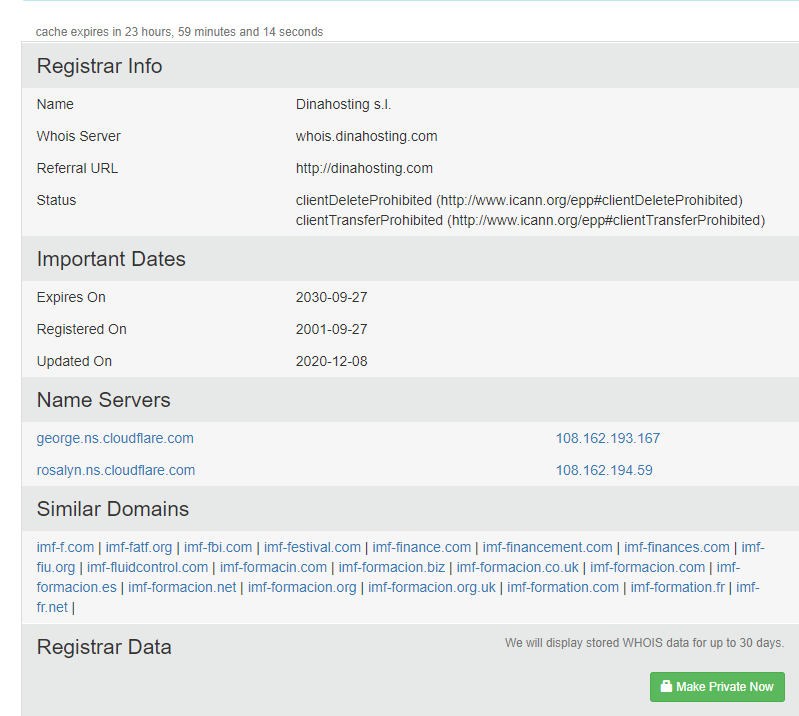
\includegraphics[scale=0.8]{./imagenes/whois}
    \caption{Who is}
\end{figure}

Además de un histórico de las IP que han sido asociadas.

\begin{figure}[h]
    \centering
    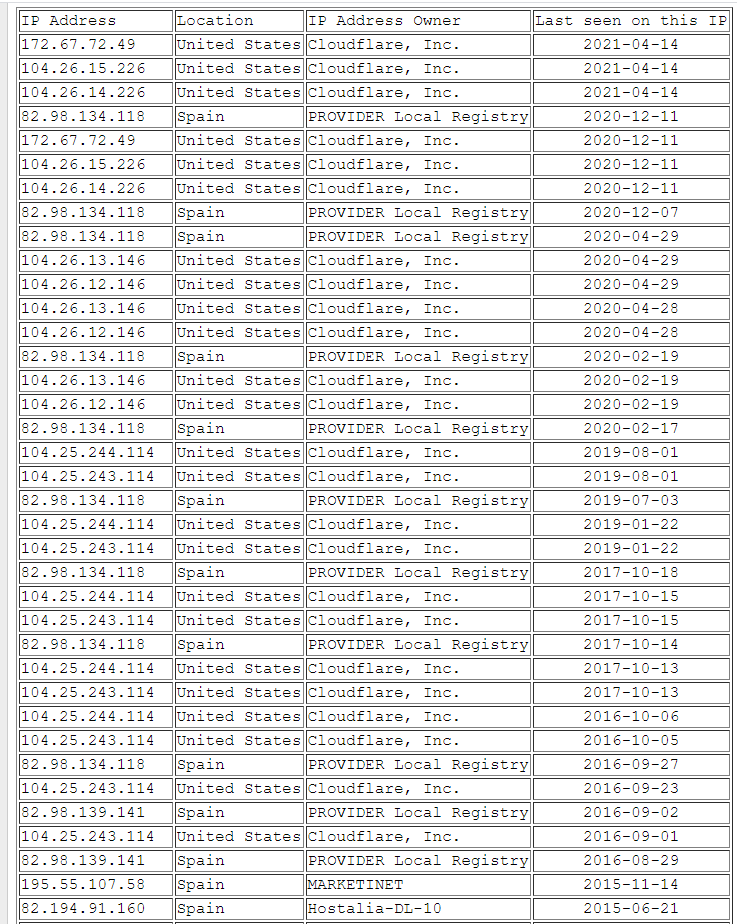
\includegraphics[scale=0.7]{./imagenes/historico_ip}
    \caption{Historial de IPs}
\end{figure}

\subsection{Harverster}
Probaremos ahora con con theHarvester pra buscar información en páginas como Google o Linkedin. También se podría buscar cuentas asociadas en Facebook, Twitter...\\
Encontramos en Google diferentes emails asociados a la institución y dos hosts, con su  IP asociada.
\begin{figure}[h]
    \centering
    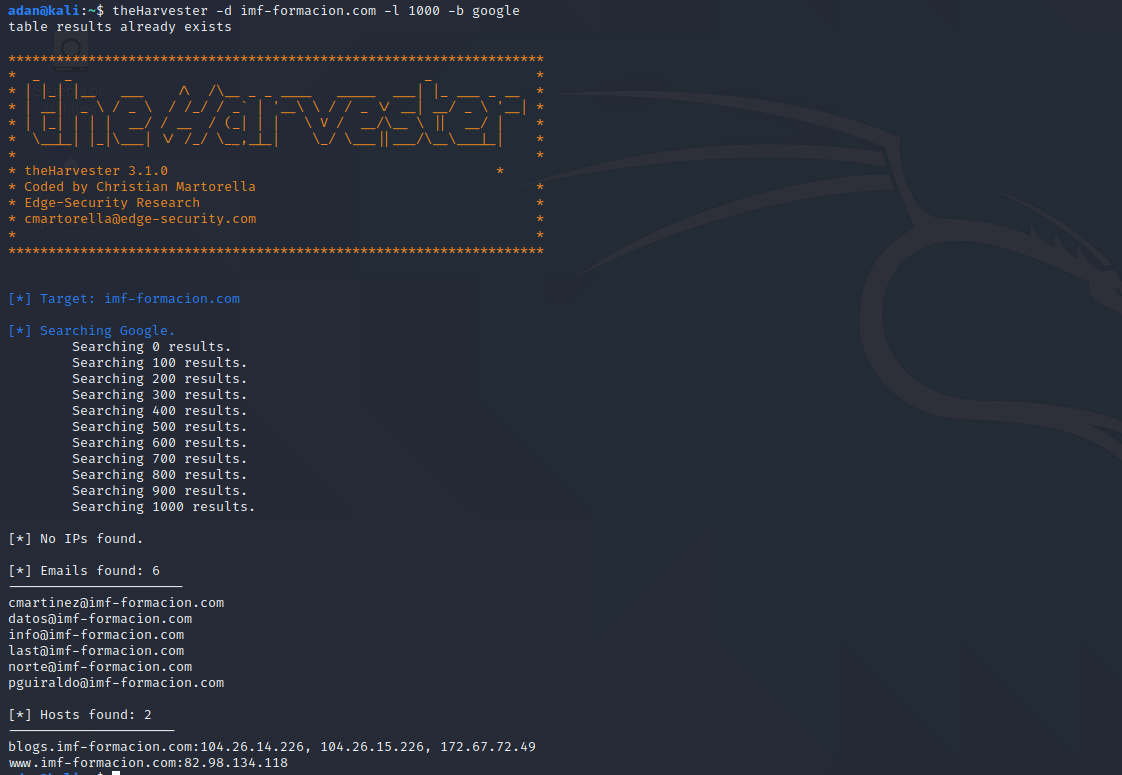
\includegraphics[scale=0.7]{./imagenes/harvester}
    \caption{TheHarvester en Google}
\end{figure}

Si escaneamos Linkedin, obtendremos:

\begin{figure}[h]
    \centering
    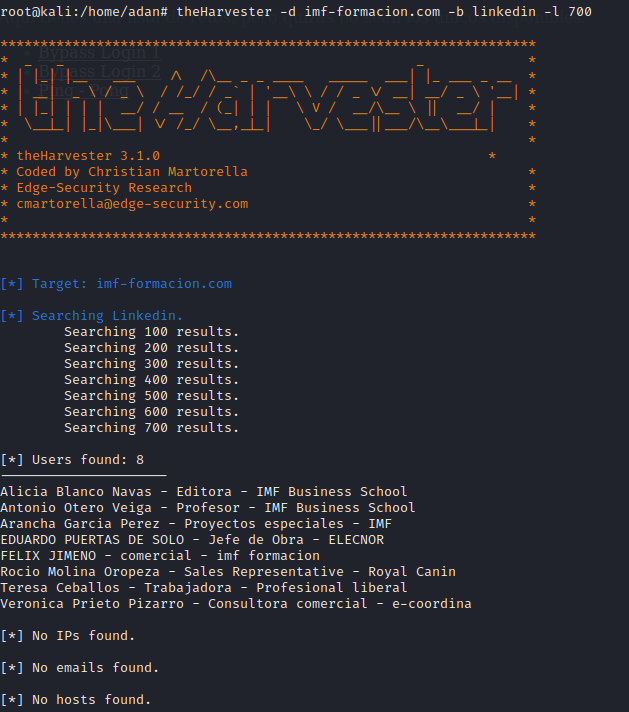
\includegraphics[scale=0.6]{./imagenes/harvester_linkedin}
    \caption{TheHarvester en LinkedIn}
\end{figure}

Esta información podría ser valiosa de cara a ataques de ingeniería social. 

\subsection{NMAP}
Podemos también ver qué servicios o puertos están abiertos en la página, usando nmap.

\begin{figure}[h]
    \centering
    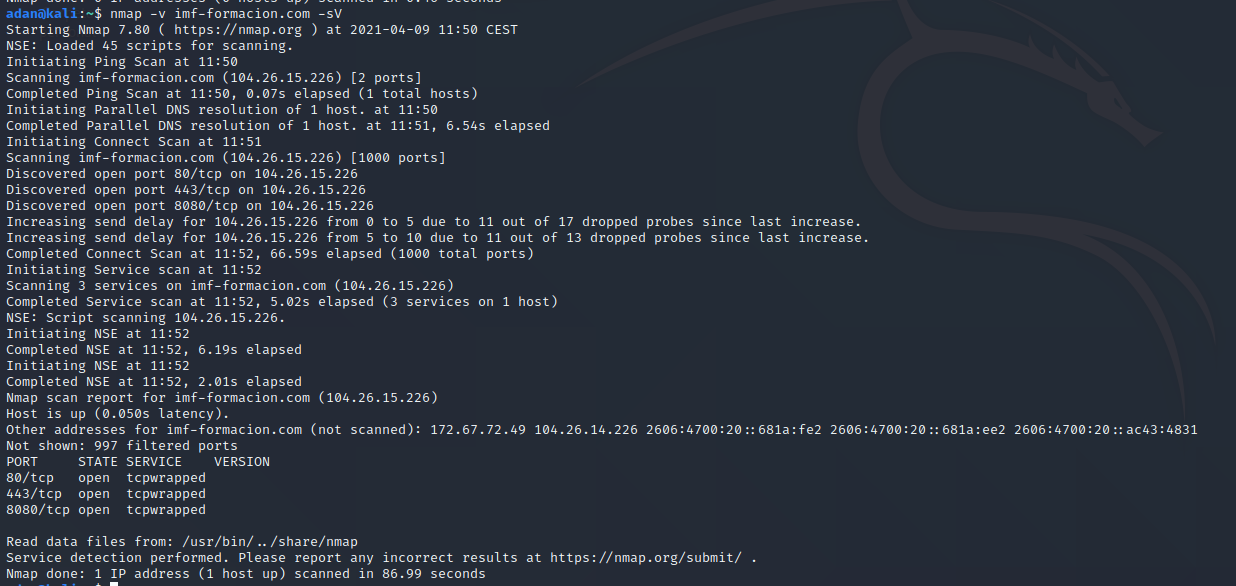
\includegraphics[scale=0.5]{./imagenes/nmap}
    \caption{Resultado de nmap.}
\end{figure}

Viendo que los puertos 80, 443 y 8080 están abiertos.
%--------------------------------%--------------------------------%--------------------------------
%--------------------------------%--------------------------------%--------------------------------
\newpage
%--------------------------------%--------------------------------%--------------------------------
%--------------------------------%--------------------------------%--------------------------------
\section{Análisis de vulnerabilidades}

Analizaremos ahora las vulnerabilidades de la web, pero en este caso lo haremos sobre la máquina virtual. En primer lugar, con el comando \textbf{netdiscover}, encontraremos la IP donde está alojada la máquina.
\newpage
\begin{figure}[h]
    \centering
    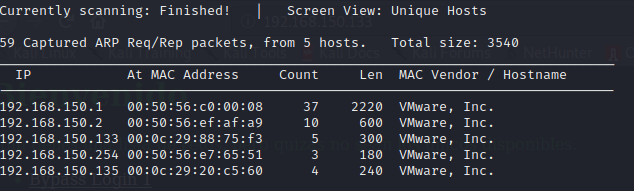
\includegraphics[scale=0.2]{./imagenes/escaneo_red}
    \caption{Escaneo de la red}
\end{figure}



\subsection{WhatWeb}
Con WhatWeb, podemos encontrar información sobre el servidor Apache, y con ello buscar posibles vulnerabilidades. En este caso, se buscan en las flags y son explotadas.

\begin{figure}[h]
    \centering
    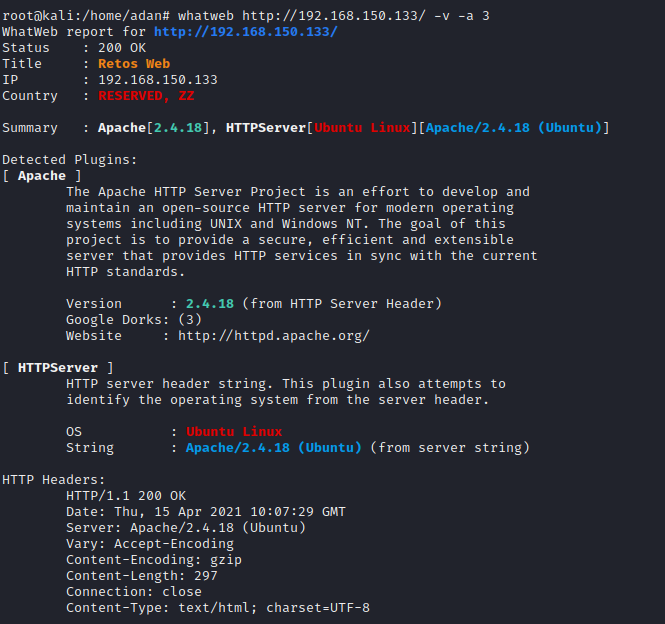
\includegraphics[scale=0.3]{./imagenes/whatweb}
    \caption{Resultado de Whatweb}
\end{figure}

\subsection{NMAP ANALISIS}
Para un análisis más exhaustivo de los servicios, usaremos \textbf{nmap} con \textbf{-sV} para obtener mayor información.
\begin{figure}[h]
    \centering
    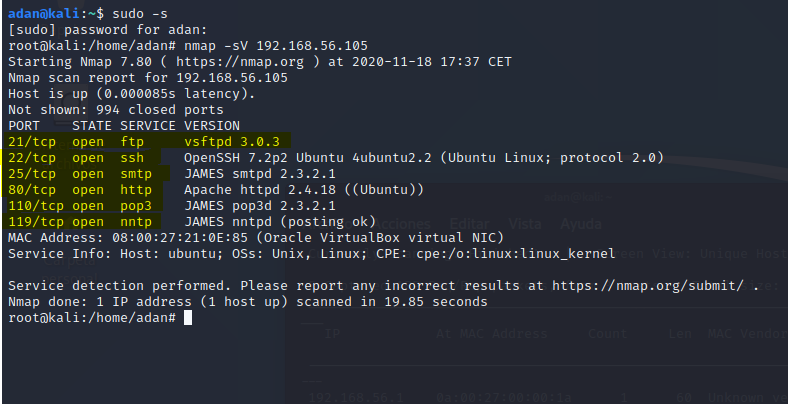
\includegraphics[scale=0.7]{./imagenes/nmap_maquina}
    \caption{Resultado de nmap}
\end{figure}
Los servicios de Apache y FTP serán explotados después, así que los obviaremos. Sí que podemos hacer una valoración más exhaustiva de las versiones de SSH y de James.

\subsection{SSH}
Centramos la búsqueda en el servicio SSH, y podemos encontrar un exploit para esa versión que nos permite la enumeracion de usuarios, pero que no vamos a exploitear. 
\begin{figure}[h]
    \centering
    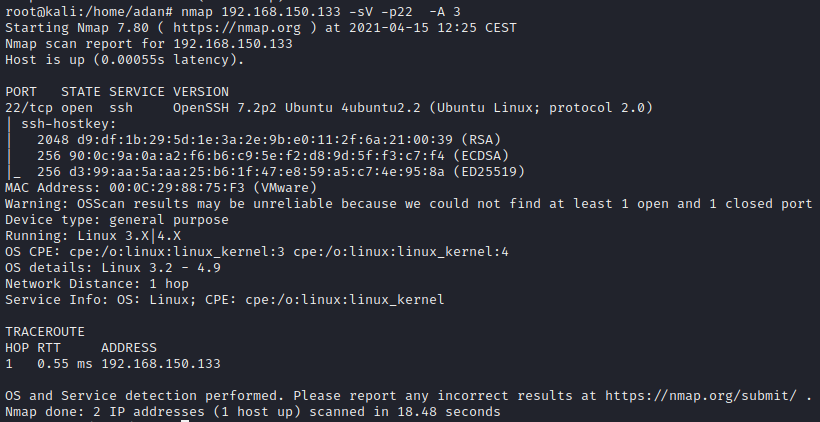
\includegraphics[scale=0.7]{./imagenes/nmap_ssh}
    \caption{Resultado de nmap ssh}
\end{figure}

\begin{figure}[h]
    \centering
    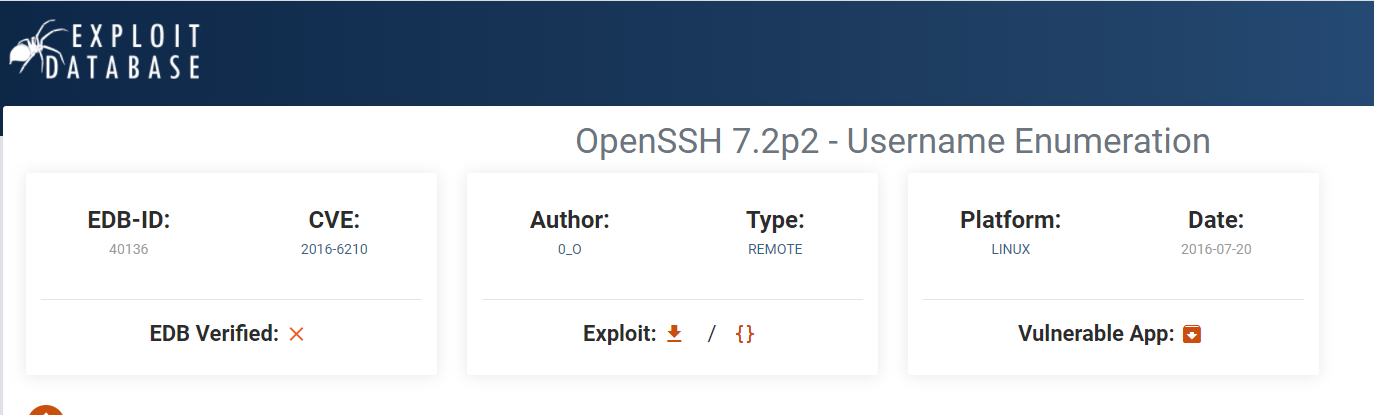
\includegraphics[scale=0.7]{./imagenes/exploit_ssh}
    \caption{Resultado de nmap ssh}
\end{figure}

\subsection{James}
En este caso, no hay ningún exploit aparente para la versión, pues han sido parcheados y este no parece ser un vector de entrada.
% -------------------------------------------------
% -------------------------------------------------
% -------------------------------------------------
% -------------------------------------------------
% -------------------------------------------------

\section{Análisis de vulnerabilidades.}
Procedemos, tras el reconocimiento, a buscar las diez flags del servidor. 
% -------------------------------------------------% -------------------------------------------------
\subsection{index.html}

Una vez hemos encontrado la IP donde está corriendo el servidor y accedemos, nos encontramos la siguiente página, con los retos a realizar.

\begin{figure}[h]
    \centering
    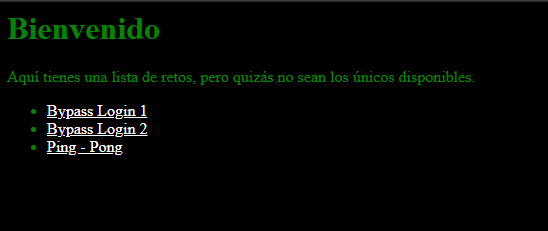
\includegraphics[scale=0.75]{./imagenes/index}
    \caption{a nice plot}
\end{figure}

En primer lugar, haremos una inspección de código, donde encontraremos la primera flag.

\begin{figure}[h]
    \centering
    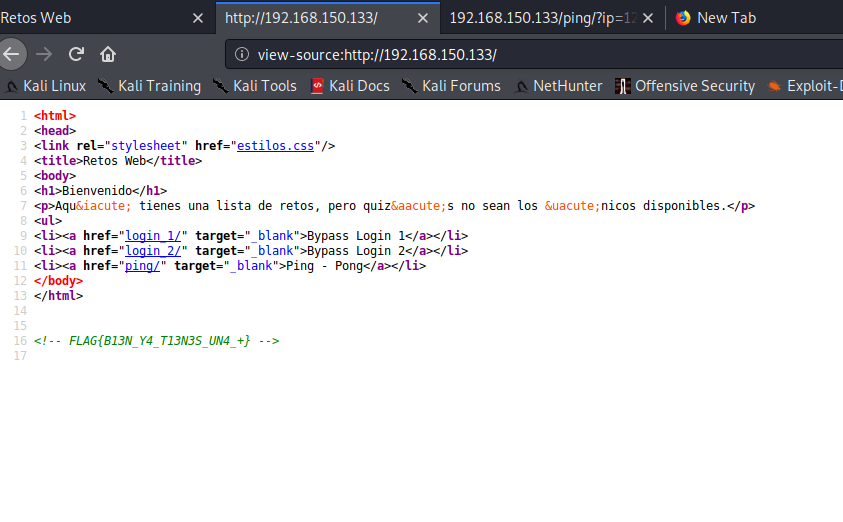
\includegraphics[scale=0.25]{./imagenes/flag_codigo_fuente}
    \caption{Flag 1}
\end{figure}



% -------------------------------------------------% -------------------------------------------------
\subsection{Login 1}

Seguidamente, accederemos al primer reto.

\begin{figure}[h]
    \centering
    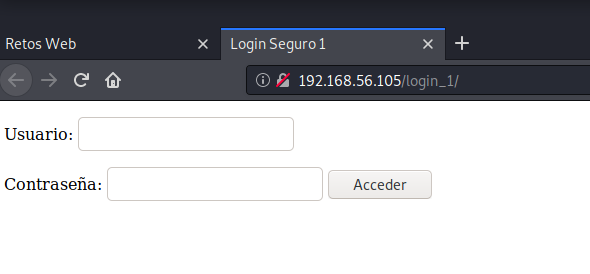
\includegraphics[scale=0.75]{./imagenes/login_1}
    \caption{Acceso al login}
\end{figure}

Como en el acso anterior, procederemos a inspeccionar el código:

\begin{figure}[h]
    \centering
    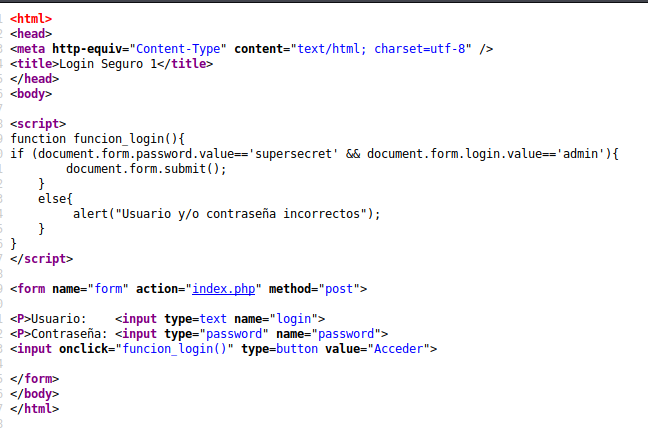
\includegraphics[scale=0.75]{./imagenes/login_1_fuente}
    \caption{Código fuente del login 1}
\end{figure}

Donde podemos encontrar el usuario y contraseña para acceder, con el que conseguiremos la siguiente flag.

\begin{figure}[h]
    \centering
    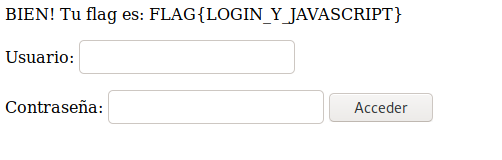
\includegraphics[scale=0.75]{./imagenes/login_1_flag}
    \caption{Flag 2}
\end{figure}


% -------------------------------------------------% -------------------------------------------------
\subsection{Login 2}

Aparentemente en este reto, hemos de hacer un bypass al login de autenticación.
Interceptamos los paquetes con wireshark y podemos ver que la Autirozacion es basic, esta en base64 y decodificándola, es admin:root. 
\begin{figure}[h]
    \centering
    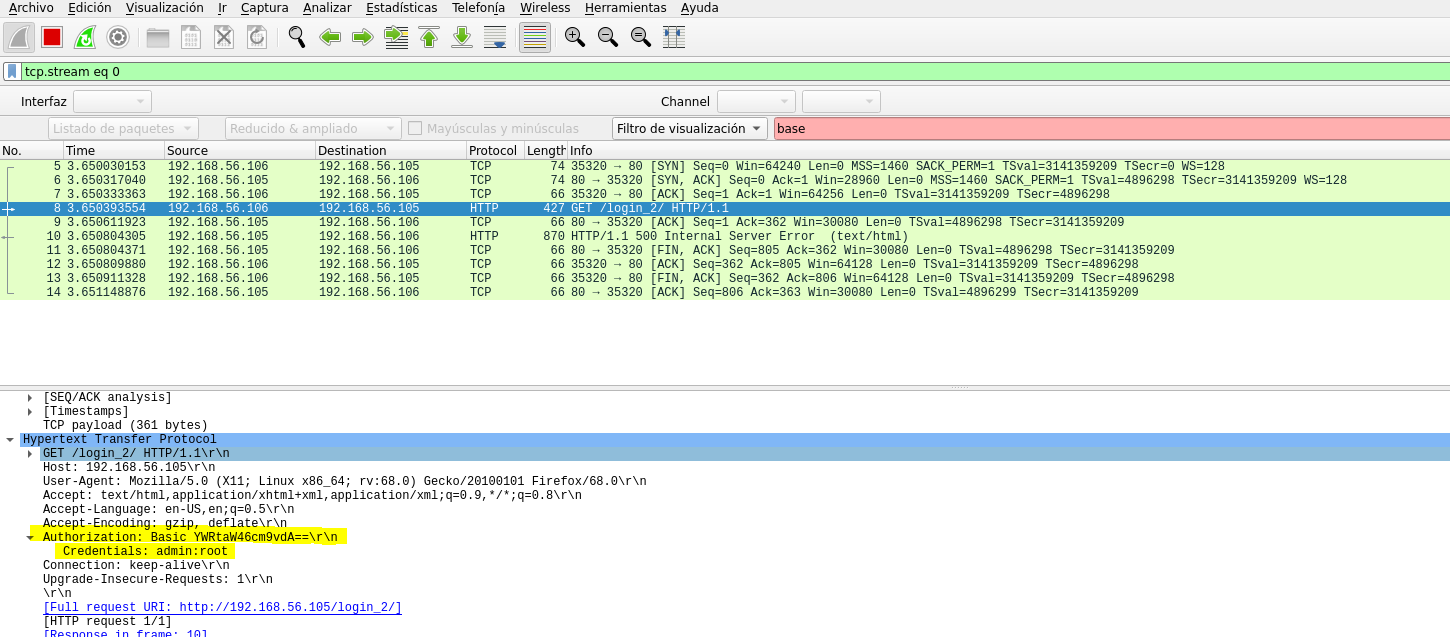
\includegraphics[scale=0.25]{./imagenes/wireshark}
    \caption{Wireshark}
\end{figure}

Sin embargo, no nos da acceso, así que probaremos utilizando el comando CURL y cambiando a una petición POST, consiguiendo acceso.

\newpage

\begin{figure}[h]
    \centering
    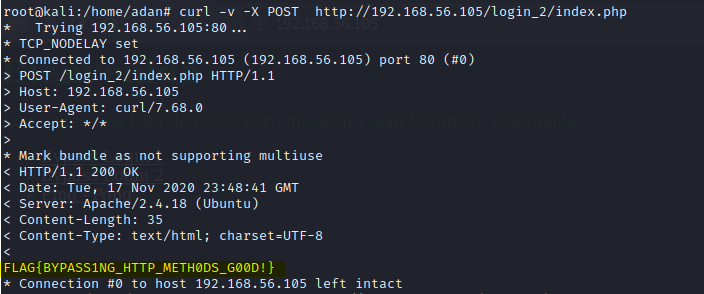
\includegraphics[scale=0.6]{./imagenes/flag_bypass}
    \caption{Flag 3}
\end{figure}

% -------------------------------------------------% -------------------------------------------------
\subsection{Robots}
Realizamos ahora una enumeración de directorios, 

\begin{figure}[h]
    \centering
    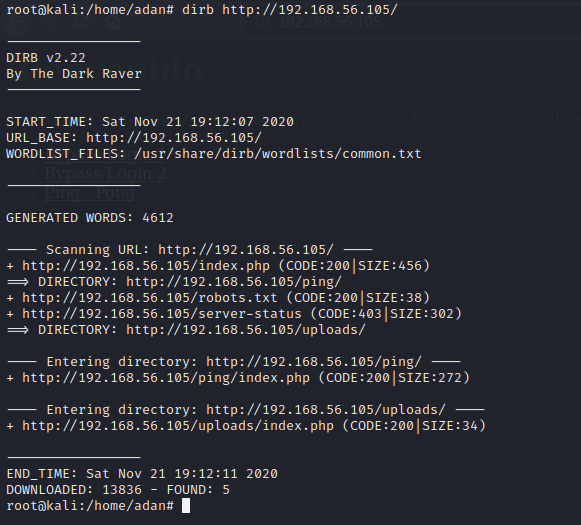
\includegraphics[scale=0.55]{./imagenes/enumera_directorios}
    \caption{Enumera directorios}
\end{figure}

Donde encontramos las páginas de rotbots.txt y uploads. Procederemos a acceder a ambas.\\
En primer lugar, accedemos a robots.txt
\begin{figure}[h]
    \centering
    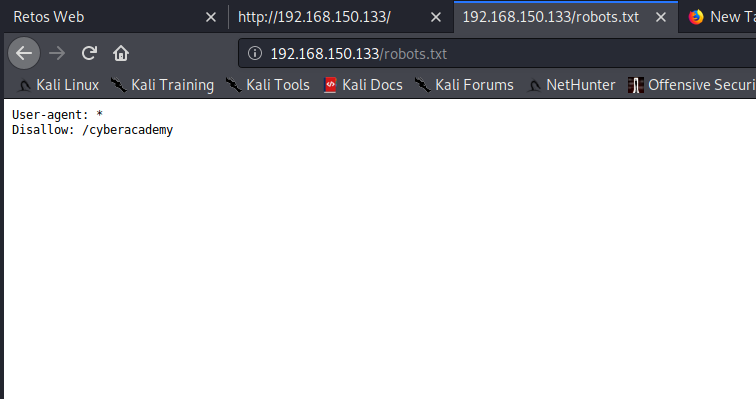
\includegraphics[scale=0.5]{./imagenes/robots_txt}
    \caption{Página de robots}
\end{figure}

Y accediendo a la ruta /cyberacademy, encontramos la siguiente flag.

\begin{figure}[h]
    \centering
    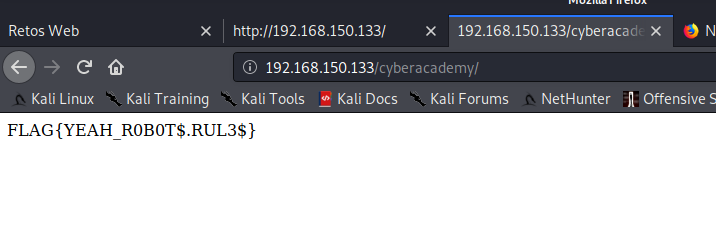
\includegraphics[scale=0.5]{./imagenes/robots_txt_flag}
    \caption{Flag 4}
\end{figure}

\newpage
% -------------------------------------------------% ------------------------------------------------
\subsection{Uploads}
Como en el paso anterior, accedemos a la carpeta de uploads, donde encontraremos la siguiente flag.

\begin{figure}[h]
    \centering
    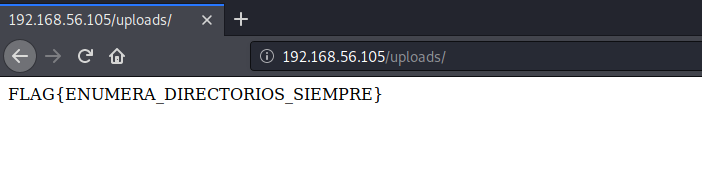
\includegraphics[scale=0.5]{./imagenes/enumera_directorios_flag}
    \caption{Flag 5}
\end{figure}

% -------------------------------------------------% -------------------------------------------------
\subsection{FTP}
En este paso, procederemos a realizar un escaneo de puertos en búsqueda de todos los posibles abiertos.

\begin{figure}[h]
    \centering
   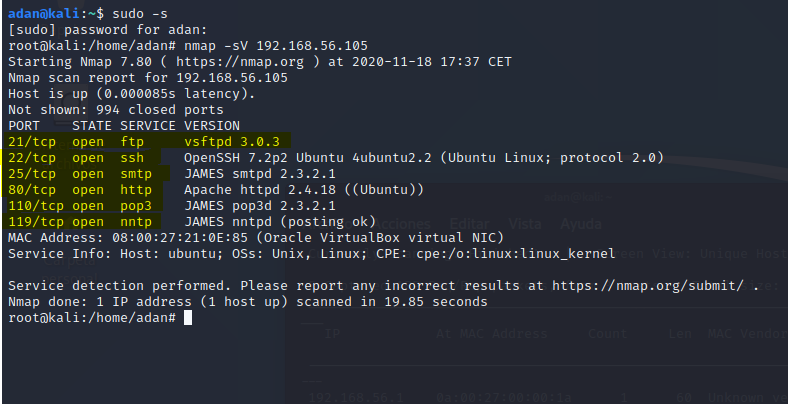
\includegraphics[scale=0.4]{./imagenes/escaneo_puertos}
    \caption{Escaneo de puertos}
\end{figure}

Empezamos con el puerto 21, haciendo un \textbf{ftp}, seguidamente nos conectamos intentando usar la contraseña por defecto ftp, y obtenemos acceso. (notar que es el usuario y contraseña que habíamos visto con wireshark) \\
Vemos que en el directorio está la flag.txt, nos la descargamos y la abrimos, obteniendo el siguiente flag.

\begin{figure}[h]
    \centering
    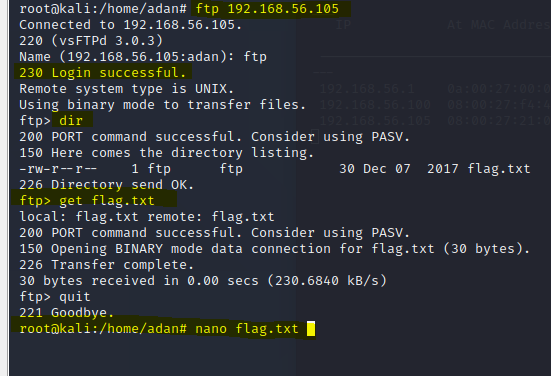
\includegraphics[scale=0.5]{./imagenes/ftp_flag}
    \caption{Flag 6}
\end{figure}


% -------------------------------------------------% -------------------------------------------------
\subsection{Ping}
En el reto de ping, ya que esta usando un GET probamos con un Command Injection, pare ver si lo ejecuta. 
\begin{figure}[h]
    \centering
    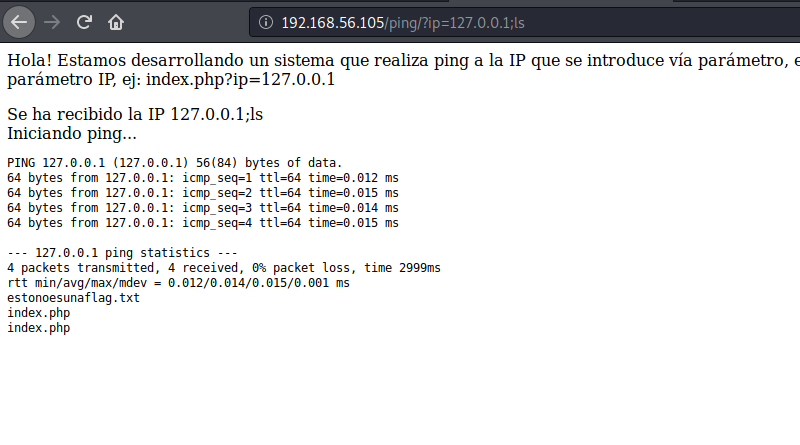
\includegraphics[scale=0.5]{./imagenes/ping}
    \caption{Command Injection en Ping}
\end{figure}

Encontramos un archivo .txt, probaremos a realizar cat por si lo podemos conseguir:

\begin{figure}[h]
    \centering
    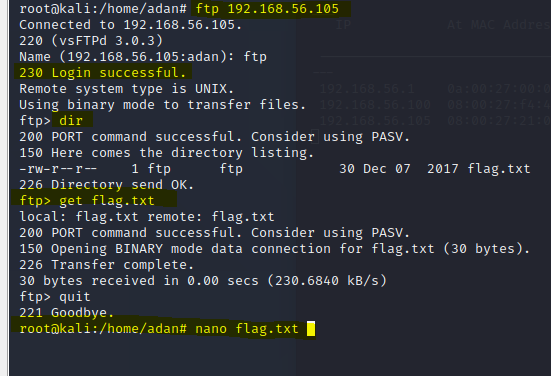
\includegraphics[scale=0.5]{./imagenes/ftp_flag}
    \caption{Flag 7}
\end{figure}
% -------------------------------------------------% -------------------------------------------------
\subsection{Deloitte y OPT}
En el siguiente paso, probaremos con el comando \textbf{find} para encontrar todos los elementos llamados "flag.txt".

\begin{figure}[h]
    \centering
    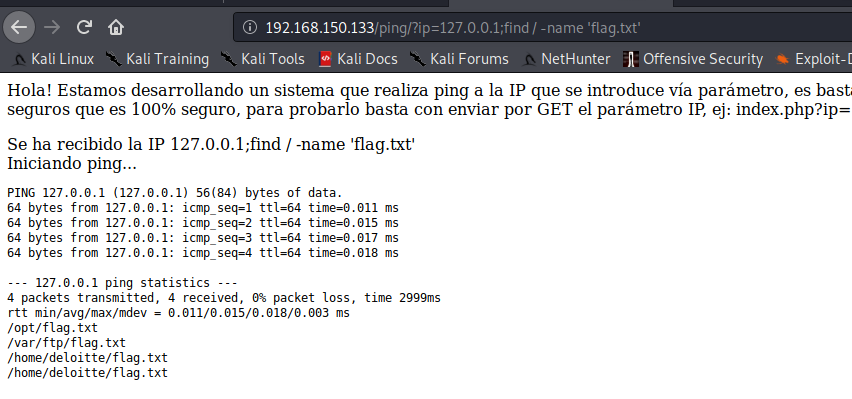
\includegraphics[scale=0.5]{./imagenes/ping_busqueda_flag}
    \caption{Búsqueda de flags}
\end{figure}

Donde encontramos que en las carpetas de /opt/ y /home/deloitte/ existen dos flags a las que podemos acceder utilizando el comando cat. 

En primer lugar accederemos a la de Deloitte.
\begin{figure}[h]
    \centering
    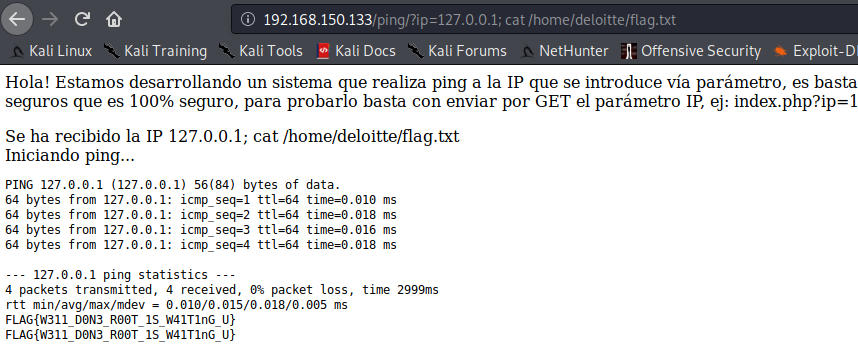
\includegraphics[scale=0.5]{./imagenes/cat_flag_deloitte}
    \caption{Flag 8}
\end{figure}

\newpage

Y después la de opt.

\begin{figure}[h]
    \centering
    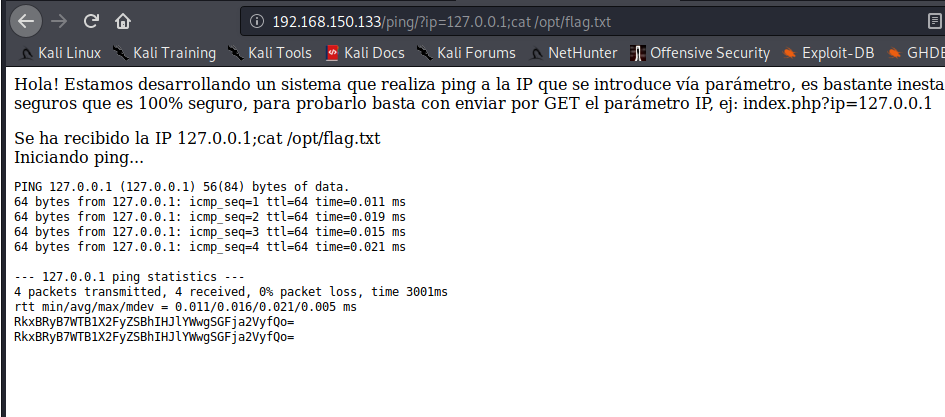
\includegraphics[scale=0.4]{./imagenes/cat_flag_opt}
    \caption{OPT, flag encriptada.}
\end{figure}

La flag de /opt/ está encriptada en base64, lo convertimos en texto legible y obtenemos la flag esperada.

\begin{figure}[h]
    \centering
    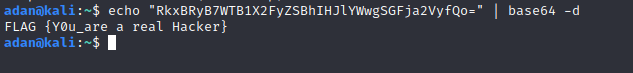
\includegraphics[scale=0.4]{./imagenes/flag_opt}
    \caption{Flag 9}
\end{figure}

\newpage 

% -------------------------------------------------% -------------------------------------------------
\subsection{Escalada de privilegios}
Procederemos en el último paso a realizar una escala de privilegios. Como en la página ping podemos ejecutar código, aseguramos que la máquina tiene python instalada. En nuestra terminal, utilizamos el comando \textbf{nc -lvp 1234}, por otro lado, ejecutamos el código adecuado en la máquina atacada: 

\begin{figure}[h]
    \centering
    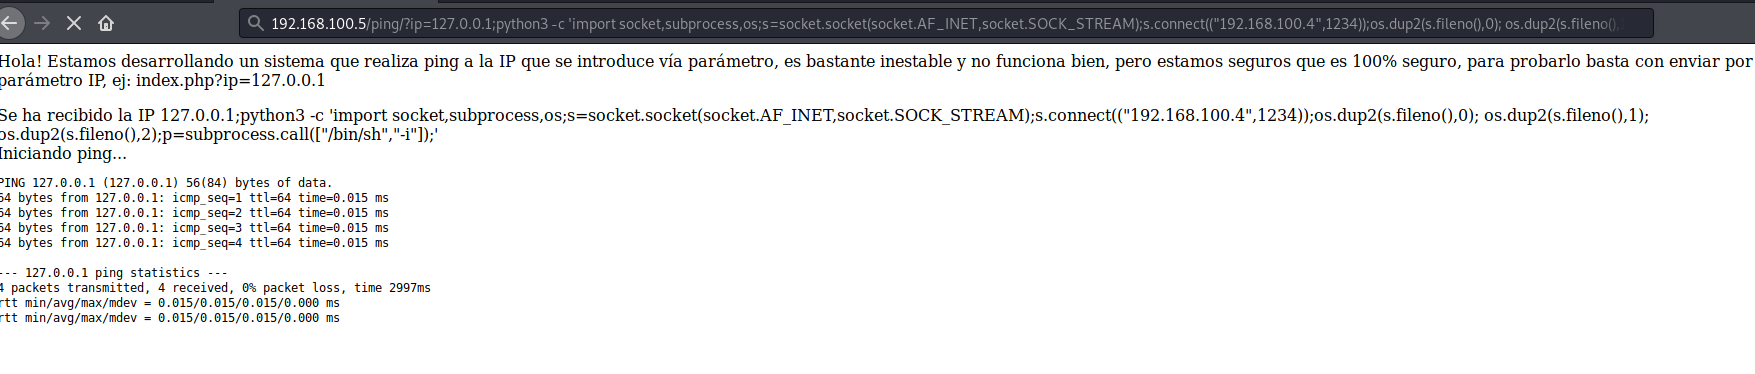
\includegraphics[scale=0.25]{./imagenes/ejecucion_codigo}
    \caption{Código en la máquia atacada}
\end{figure}

En la máquina atacante, obtendremos acceso, y con \textbf{uname -a} veremos la versión del linux para buscar el exploit adecuado.
\begin{figure}[h]
    \centering
    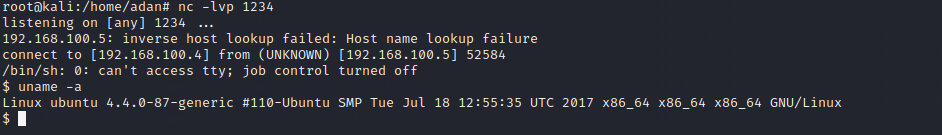
\includegraphics[scale=0.45]{./imagenes/maquina_atacante}
    \caption{Resultado en la máquina atacante}
\end{figure}

Con la información obtenida, buscamos el exploit a usar (tras varios fallidos) y encontramos el siguiente

\begin{figure}[h]
    \centering
    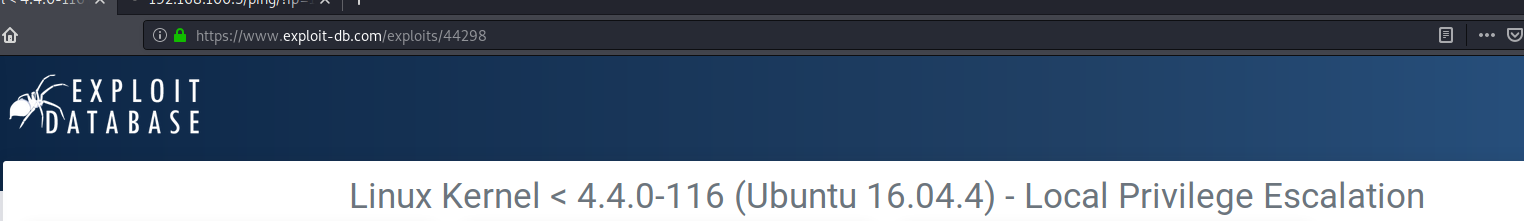
\includegraphics[scale=0.25]{./imagenes/exploit_a_usar}
    \caption{Exploit que usaremos}
\end{figure}

Para subir el exploit, haremos lo suiguiente:
\begin{enumerate}
    \item Bajar y compilar el exploit. 
    \item Crear un servidor apache.
    \item Subir el exploit compilado a nuestro servidor, en la carpeta /var/www/
\end{enumerate}
\newpage
\begin{figure}[h]
    \centering
    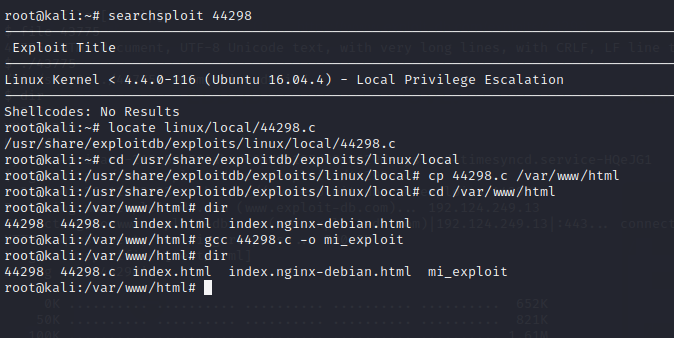
\includegraphics[scale=0.5]{./imagenes/subir_exploit_a_server}
    \caption{Subida de exploit al servidor}
\end{figure}

Como somos el usuario www-data, tenemos solo permisos en la carpeta /tmp. Así pues, nos moveremos a esa carpeta y descargaremos el exploit con wget. Seguidamente le damos permisos de ejecución  al exploit y lo ejecutamos.

\begin{figure}[h]
    \centering
    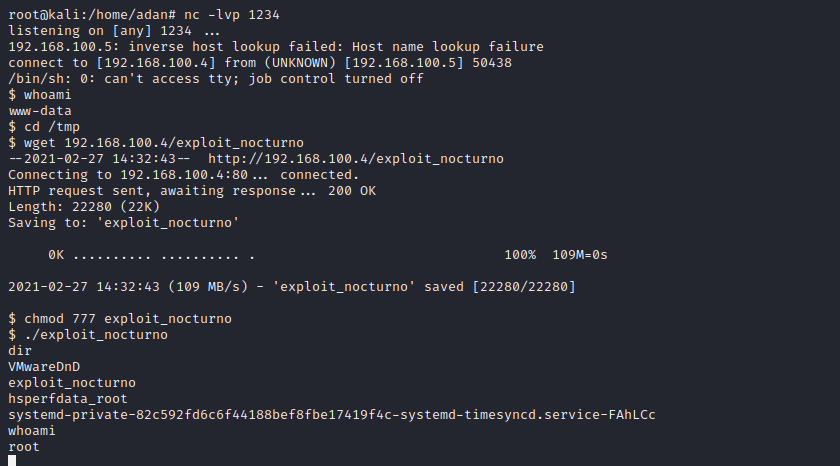
\includegraphics[scale=0.5]{./imagenes/ejecucion_exploit}
    \caption{Obtención de privilegios}
\end{figure}

Y comprobamos finalmente que hemos obtenido tanto la escalada de privilegios como la última flag.

\begin{figure}[h]
    \centering
    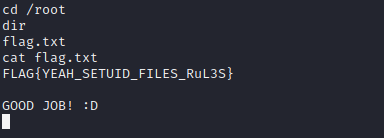
\includegraphics[scale=0.7]{./imagenes/flag_root}
    \caption{Flag 10}
\end{figure}





% -------------------------------------------------% -------------------------------------------------








\end{document} 
